\chapter{Introdução ao Projeto}
\label{chapter:intro}

O cenário atual do desenvolvimento tecnológico encontra-se no meio de uma quarta revolução industrial. Nunca se produziu tantos dados e se utilizou redes como a própria internet para propaga-los. É de se esperar que tanto a academia e diferentes mercados demandem inovações para o compartilhamento desses dados em tempo real ou próximo disso. Aquecendo o mercado que engloba transporte, análise e inteligência de dados.

Este projeto propõe uma interface para comunicação entre as diferentes tecnologias e camadas de rede, de forma que o desenvolvedor só se preocupe em  implementar e configurar uma interface para mapear a melhor opção de ferramentas para a aplicação. O projeto lida com protocolos baseados na pilha TCP/IP, uma unanimidade em redes conectadas a internet. Podendo se estender para outras protocolos de aplicações de escopo fechado. O foco está no protocolo de aplicação MQTT (\textit{Message Queuing Telemetry Transport}) \cite{mqtt}, um protocolo que opera sobre o TCP/IP, leve e extremamente utilizado para compartilhamento dados telemétricos, de estado e de pequenas mensagens. Oferecendo uma API para aquisição, transmissão, recepção e armazenamento de dados telemétricos..

A Internet das Coisas é a rede que permite a conexão e compartilhamento de dados  de dispositivos físicos . Ela é derivada de métodos de comunicação entre máquinas e telemetria. Pode ser dissecada em três camadas de aquisição, comunicação e aplicação  podendo ser implementada utilizando diversos protocolos de comunicação, dependendo da tecnologia disponível. É importante que sistemas IoT sejam projetados de forma a atender a aplicação eficientemente, porém tal tarefa não é fácil nem simples. Este projeto oferece uma interface que permite facilitar tal tarefa.

\section{Internet das Coisas}
\label{section:iot}

"A Internet das Coisas tem o potencial de mudar o mundo. Assim como a Internet fez. Talvez até mais" \cite{ashton:iot}. Uma tradução livre de Rampim \cite{Rampim:iot} da frase de Kevin Ashton, cofundandor do Auto-ID Center, em 1999. Apesar de ser um nome feito somente para chamar atenção, foi a primeira citação da expressão Internet das Coisas, e de lá vingou.

No contexto da Indústria 4.0, encontra-se a internet das coisas ou IoT, responsável por estruturar as aplicações de aquisição, transmissão e armazenamento de dados a serem analisados. Não é uma surpresa que a Internet das Coisas envolva áreas como eletrônica, computação e telecomunicações em um pacote só. De fato as camadas de IoT são mundos diferentes interligados a um propósito: transmitir dados sobre um dispositivo e/ou para um dispositivo em tempo real. Segundo a Cisco IBSG, Cisco Internet Business Solutions Group \cite{cisco:ibsg}, há mais objetos conectados que pessoas no mundo, fazendo com que o ano de 2009 seja considerado o ano de nascimento da IoT.

Pode-se definir IoT como a estrutura que comunica dispositivos em rede, permitindo a transmissão de dados sobre eles em tempo real. Essa estrutura permite a troca de informações sobre um dispositivo, qual seu estado, seu desempenho, suas condições físicas e do ambiente ao seu redor. Mas, para que este ciclo esteja completo são necessárias camadas que desempenham tarefas específicas, para que o dado chegue a quem ou a o que o está esperando.

\section{Visão geral de uma aplicação IoT}
\label{section:overview}

Na \ref{fig:1.1.0/iot_app} ilustrada, temos uma rede de N sensores que enviam dados telemétricos e M atuadores que recebem ordens para executar uma função, todos estão em rede e podem receber e enviar informação em tempo real. O servidor, que pode ser um Broker como será descrito adiante neste trabalho, encaminha os dados (ou mensagens) para o banco de dados. O Banco é utilizado para análise dos dados, o controlador por sua vez envia as mensagens de decisões baseada na análise de dados a serem transmitidas para os atuadores.

\begin{figure}[h!]
\centering
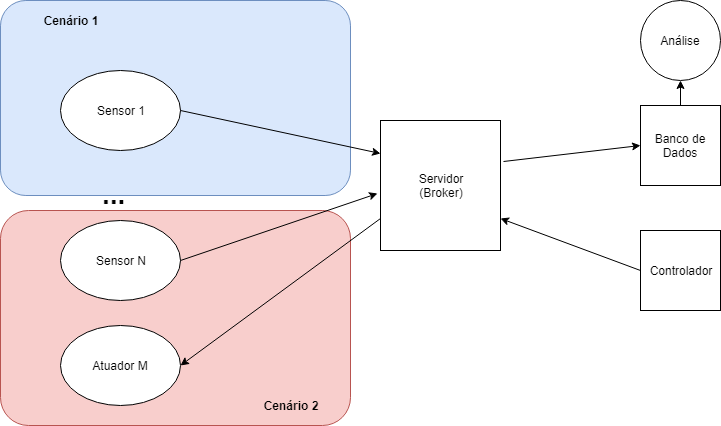
\includegraphics[width=10cm]{./02_Capitulos/02_Cap1/figures/iot_app}
\caption{Um exemplo de aplicação IoT que percorre os problemas a solucionar}
\label{fig:1.1.0/iot_app}
\end{figure}

O sensor 1 está imerso em um ambiente com usas próprias características físicas e de rede, isso ocorre com todos, isto é cada sensor está imerso num cenário próprio, variando de redes com poucos sensores a redes com grande fluxo de dados, sujeito a congestionamento. Assim, seria de grande ajuda que o  sistema se ajustasse aos diferentes cenários.

Este trabalho visa implementar um sistema que utiliza o protocolo de aplicação MQTT, para transmissão de dados em tempo real entre dispositivos). O sistema contempla também persistência de dados utilizando banco de dados MongoDB, com o diferencial de se adaptar a cenários através de canais de dados chamados Data Streams, oferecendo diferentes configurações que podem otimizar o envio de dados em cada cenário.

\begin{figure}[h!]
\centering
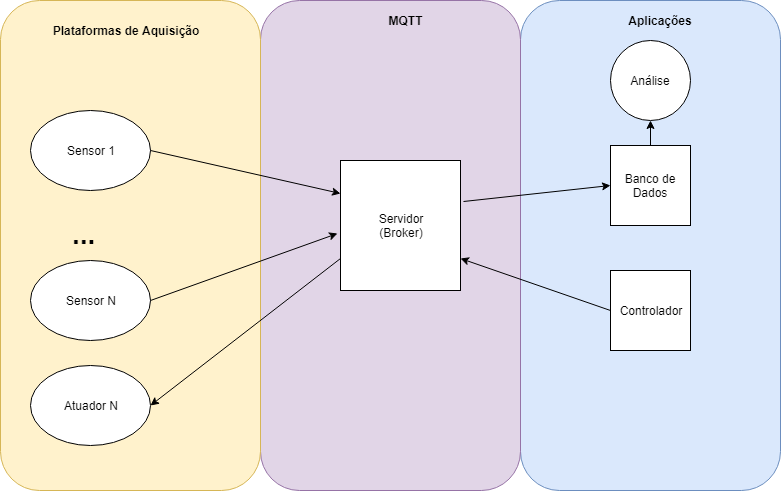
\includegraphics[width=10cm]{./02_Capitulos/02_Cap1/figures/iot_app-layers}
\caption{A aplicação dividida em blocos exercendo um papel em uma aplicação IoT}
\label{fig:1.1.0/iot_app-layers}
\end{figure}


Cada bloco é responsável por uma tarefa no sistema IoT, da aquisição de dados a persistência destes, conforme ilustrado na \ref{fig:1.1.0/iot_app-layers}. Para entender melhor cada tarefa, será descrito o projeto e as implementações em cada bloco no sistema.

\section{As Camadas da IoT}
\label{section:camadas_iot}

Uma rede IoT pode ser divida em camadas que exercem funções específicas no transporte de dados, de uma forma semelhante a redes de computadores, a camada acima não precisa saber como a inferior funciona, formando uma estrutura de pilha como na figura \ref{fig:1.2.0/camadas_iot}.

\begin{figure}[h!]
\centering
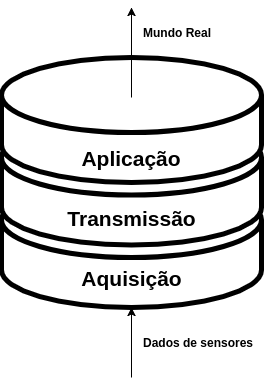
\includegraphics[width=5cm]{./02_Capitulos/02_Cap1/figures/iot_stack}
\caption{As três camadas do IoT, dos sensores ao mundo real}
\label{fig:1.2.0/camadas_iot}
\end{figure}

A primeira camada é a de aquisição de dados, que lida com o mundo físico e captura estes dados através de sensores e conversores A/D, também realiza o processamento para entregar em um formato adequado para transmissão e inteligível do outro lado, dependo da aplicação. A segunda camada é a camada de transmissão, na qual estão, efetivamente, as camadas de rede embutidas. Como o nome já denuncia, ela lida com os aspectos de rede e comunicação para que o dados cheguem seus destinos. E por último temos a camada de aplicação, a mais abrangente e que envolve maior poder computacional. Ela recebe os dados e lida com os processos de aplicação destes dados, seja análise, visualização, armazenamento ou a estruturação dos mesmos.

\subsection{Aquisição}
\label{subsection:aquisicao}

A etapa de aquisição está inserida diretamente no contexto de dados físicos, geralmente são hardwares menos complexos, focados em processamento de dados e entrada e saída com conversão analógico-digital. Se comunicam com sensores ou centrais de controle lógico. São responsáveis por:

\begin{itemize}
	\item Receber dados de sensores;
	\item Conversão A/D;
	\item Processamento de valores;
	\item Envio de dados em tempo real;
\end{itemize} 

Para atender essas tarefas, não é necessário grande poder de processamento, microcontroladores ou microprocessadores são capazes de atender aos requisitos necessários para uma grande gama de variáveis físicas, se acompanhados de módulos de rede e portas I/O, assim como a implementação do software. Serão vistos dois exemplos desses dispositivos, que utilizam tanto MCU  e outro um Consoles com Sistemas Operacionais leves.
 

\subsection{Transmissão}
\label{subsection:transmicao}

Esta camada é o coração do IoT. A transmissão define quais dispositivos eletrônicos e suas especificação técnicas. Também define como os softwares da camada de aplicação e aquisição devem ser implementados baseado na estrutura da pilha de rede que será usada para transmitir.

Na próxima seção, a camada de rede e suas formas de implementação serão detalhadas. É importante que esta camada seja definida da melhor forma a atender sua aplicação, alguns aspectos relevantes nesse sentido são:: 
\begin{itemize}
\item Quantidade de dados transmitido;
\item Número de acessos; 
\item Distância entre dispositivos;
\item Segurança;
\end{itemize}

\subsection{Aplicação}
\label{subsection:aplicacao}

A camada de aplicação encabeça a pilha do IoT. É ela que de fato trata os dados. Ela disponibiliza os dados para o mundo real, podendo exercer múltiplas funções simultâneas incluindo:

\begin{itemize}
\item Armazenamento e Análise; Através de Bancos de Dados e Aplicações;
\item Visualização; Aplicações Web, disponibilizando gráficos e tabelas de dados;
\item Inteligência e aprendizado; Machine Learning e Estatística para decisões e classificação;
\item Serviços e servidores; Aplicações em nuvem fornecendo microserviços em aplicações Web;
\end{itemize}

Nesta camada estão presentes as pontas apontados pela camada de aquisição, assim como os servidores que gerenciam os clientes (geralmente implementados na camada de aquisição) e serviços e configurações oferecidos pelo sistema em si.

\section{Redes de Computadores}
\label{section:camadas_de_rede}

Como visto anteriormente, a camada de transmissão basicamente define a infraestrutura do sistema. Ela é construída baseada em como a rede é implementada. Redes de computadores são complexas com diferentes aspectos a se preocupar. Dividir em camadas permite modularizar a implementação da rede, de modo que cada camada tenha uma tarefa na estrutura de comunicação dos aspectos físicos ao software. Como uma camada  não precisa saber os detalhes e especificações da camada logo abaixo. Existem diversas formas de implementação de camadas, mas todas se baseiam em um modelo de referência, o modelo OSI \cite{Zimmermann:1988:ORM:59309.59310}.


\begin{figure}[h!]
\centering
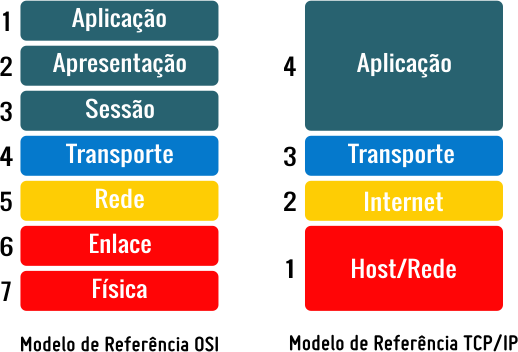
\includegraphics[width=8cm]{./02_Capitulos/02_Cap1/figures/modelo_osi_tcpip}
\caption{Diferenças entre OSI e TCP/IP em suas camadas}
\label{fig:1.2.0/modelo_osi_tcpip}
\end{figure}

Baseado no modelo OSI, temos o modelo TCP/IP \cite{TCPIP}, visualizado na \ref{fig:1.2.0/modelo_osi_tcpip} e utilizado na internet e base para protocolos de aplicação muito utilizados como HTTP, WebSocket e MQTT. Em ambos cada camada exerce uma tarefa com seu respectivo protocolo. O protocolo define regras e convenções para a comunicação entre dispositivos em rede. A \ref{table:1.2.0} resume os detalhes de cada camada.

\begin{table}[h]
\centering
\caption{As camadas e e suas funções}
\begin{tabular}{|l|l|}
\hline
\multicolumn{1}{|c|}{CAMADA} & \multicolumn{1}{c|}{DETALHES}                                                  \\ \hline
7 - Aplicação                & Define instruções específicas da aplicação          						    \\ \hline
6 - Apresentação             & Formatação dos dados, conversão dos dados                     					\\ \hline
5 - Sessão                   & Negociação e conexão com outros nós.                                \\ \hline
4 - Transporte               & Oferece métodos para a entrega de ponta-a-ponta                        			\\ \hline
3 - Rede                     & Roteamento e endereçamento de pacotes em uma ou várias redes                                 \\ \hline
2 - Enlace                   & Detecção de erros, transmissão e recepção de quadros e controle de fluxo.                                                          \\ \hline
1 - Física                   & Aspectos físicos da transmissão \\ \hline
\end{tabular}
\label{table:1.2.0}
\end{table}


O projeto lidará com aspectos e protocolos da camada de Aplicação. Apesar de diferentes tecnologias utilizarem diferentes camadas abaixo, serão especificas características de protocolos construídos sobre o TCP/IP, por seu uso na internet e redes industriais, e que sejam eficientes em trocas de mensagens em tempo real.

